\documentclass[crop,tikz]{standalone}

\usepackage[utf8]{inputenc}

% 'crop' is the default for v1.0, before it was 'preview'
%\usetikzlibrary{...}% tikz package already loaded by 'tikz' option

\newcommand{\bracs}[1]{\left( #1 \right)}
\newcommand{\eps}{\varepsilon}
	
\begin{document}

	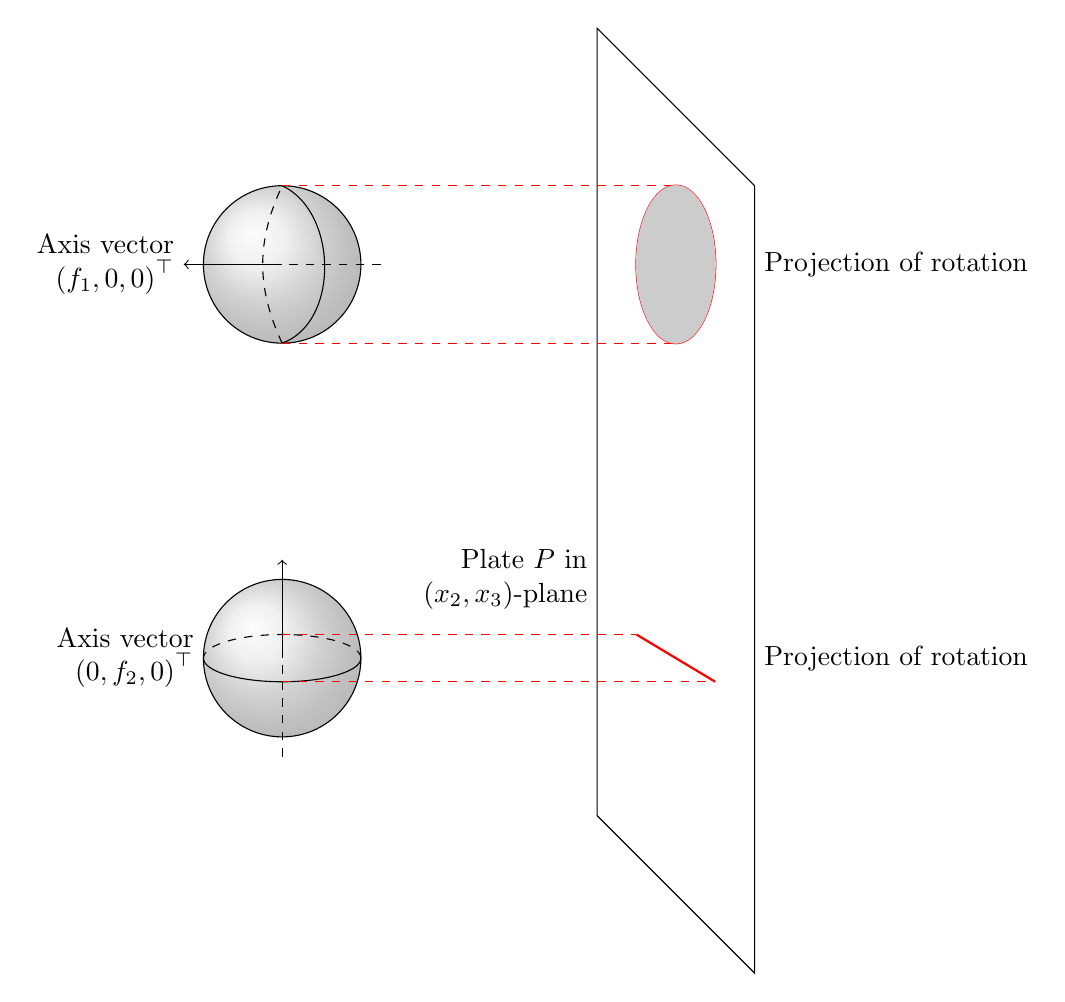
\begin{tikzpicture}
		%draw the plate itself as a parallelogram to induce a 3D effect
		\begin{scope}[shift={(4,0)}]
			\draw (0,0) -- (2,-2) -- (2,8) -- (0,10) -- cycle;
		\end{scope}
		
		%the ``infinitesimally small" sphere tilted on it's axis, perpendicular to the plane
		\begin{scope}[shift={(0,7)}, scale=0.5]
		  	\shade[ball color = gray!40, opacity = 0.4] (0,0) circle (2cm);
  			\draw (0,0) circle (2cm);
			\draw (0,-2) to[in=335, out=20] (0,2);
			\draw[dashed] (0,-2) to[in=245, out=115] (0,2);
  			%axis of rotation (perp to plane)
  			\draw[dashed] (2.5,0) -- (0,0);
  			\draw[->] (0,0) -- (-2.5,0);
		\end{scope}
		%now draw it's projection onto the plane...
		\begin{scope}[shift={(0,7)}]
			\draw[red, dashed] (0,1) -- (5,1);
			\draw[red, dashed] (0,-1) -- (5,-1);
%			\draw (5,-1) to[in=290, out=65] (5,1) to[in=205, out=115] cycle;
			\begin{scope}[xscale=0.5]
				\draw[red, thick] (2*5,0) circle (1cm);
				\filldraw[black!20!white] (2*5,0) circle (1cm);
			\end{scope}
		\end{scope}		
		
		%another ``infinitesimally small" sphere tilted on it's axis - this one is parallel to the plane (vert)
		\begin{scope}[shift={(0,2)}, scale=0.5]
		  	\shade[ball color = gray!40, opacity = 0.4] (0,0) circle (2cm);
  			\draw (0,0) circle (2cm);
  			\draw (-2,0) arc (180:360:2 and 0.6);
  			\draw[dashed] (2,0) arc (0:180:2 and 0.6);
  			%axis of rotation (|| to plane)
  			\draw[dashed] (0,-2.5) -- (0,0);
  			\draw[->] (0,0) -- (0,2.5);
		\end{scope}
		%now draw it's projection onto the plane...
		\begin{scope}[shift={(0,2)}]
			\draw[red, dashed] (0,0.3) -- (4.5,0.3);
			\draw[red, dashed] (0,-0.3) -- (5.5,-0.3);
			\draw[red, thick] (4.5,0.3) -- (5.5,-0.3);
		\end{scope}
		
		%some labels to be placed after we've moved and rescaled everything
		\node[anchor=east, align=right] at (4,3) {Plate $P$ in \\ $\bracs{x_2,x_3}$-plane};
		\node[anchor=east, align=right] at (-1,2) {Axis vector \\ $\bracs{0,f_2,0}^\top$};
		\node[anchor=east, align=right] at (-1.25,7) {Axis vector \\ $\bracs{f_1,0,0}^\top$};
		\node[anchor=west, align=left] at (6,7) {Projection of rotation};
		\node[anchor=west, align=left] at (6,2) {Projection of rotation};
	\end{tikzpicture}

\end{document}